\documentclass[12pt,table,xcolor={dvipsnames}]{beamer}
\usetheme{Pittsburgh}
\usecolortheme{seagull}
%\usepackage[utf8]{inputenc}
\usepackage{fontspec}
\usepackage{amsmath}
\usepackage{listings}
\usepackage{multirow}
\usepackage{amsfonts}
\usepackage{amssymb}
\usepackage{graphicx}
\usepackage{isabelle,isabellesym}
\author{Design and Verification of Security Protocols and Security Ceremonies}
\title{\vspace{-.2cm}Protocol Verification Techniques - Theorem Provers}
%\setbeamercovered{transparent} 
\setbeamertemplate{navigation symbols}{} 
%\logo{
\includegraphics[scale=0.015]{Brasao_UFSC.png}
\includegraphics[scale=0.2]{brasao_PPGCC.jpg}} 
\institute{Programa de Pós-Graduacão em Ciências da Computacão \\ Dr. Jean Everson Martina} 
\date{\vspace{-1cm}August-November 2016} 
\subject{} 

\newtheorem{mydef}{Definition}

\usebackgroundtemplate{
\includegraphics[width=\paperwidth,
height=\paperheight]{../reusable_images/fundo_UFSC.png}}
\begin{document}

{
\usebackgroundtemplate{
\includegraphics[width=\paperwidth,
height=\paperheight]{../reusable_images/fundo_capa.png}}
\begin{frame}
\titlepage

\includegraphics[scale=0.3]{../reusable_images/brasao_PPGCC.jpg}
\end{frame}
}

\frame{
	\frametitle{Attention!}
\begin{block}{Attention!}
This topic will be divided into two lectures. One will deal with automatic theorem provers using FOL and the second will deal with theorem provers using HOL
\end{block}
}

\frame{
\frametitle{Higher-Order Logic}
\begin{itemize}
\item Higher-order logic is a form of predicate logic that is distinguished from first-order logic by additional quantifiers and stronger semantics; \pause
\item Higher-order logics semantics are more expressive, but their model-theoretic properties are less well-behaved than those of first-order logic;\pause
\item The term "higher-order logic", abbreviated as HOL;\pause
\item HOL is any predicate logic that has greater order than Second-Order Logic;
\end{itemize}
}

\frame{
\frametitle{Higher-Order Logic}
\begin{itemize}
\item Second-Order Logic stands for the possibility of quantifying over sets;\pause
\item The idea is that you can put a quantifier over other quantifier;\pause
\item For example we can say $\forall x \exists P(x,y) \rightarrow y$\pause
\item Third-Order Logic allows for quantification over Second-Order Logic;\pause
\item Higher-order logic is the union of first-, second-, third-, …, nth-order logic;\pause
\item Higher-order logic admits quantification over sets that are nested arbitrarily deeply.
\end{itemize}
}

\frame{
\frametitle{HOL Example}
\begin{itemize}
\item First-order logic quantifies only variables that range over individuals; \pause
\item Second-order logic, in addition, quantifies over sets; \pause
\item Third-order logic also quantifies over sets of sets, and so on;\pause
\item From Second-Order Logic on we are allowed to describe mathematical induction;\pause
\item $\forall P((0\in P\land \forall i(i\in P\to i+1\in P))\to \forall n(n\in P))$\pause
\item This is the definition of the set of Natural Numbers.
\end{itemize}
}

\frame{
\frametitle{Lawrence Charles Paulson - Larry}
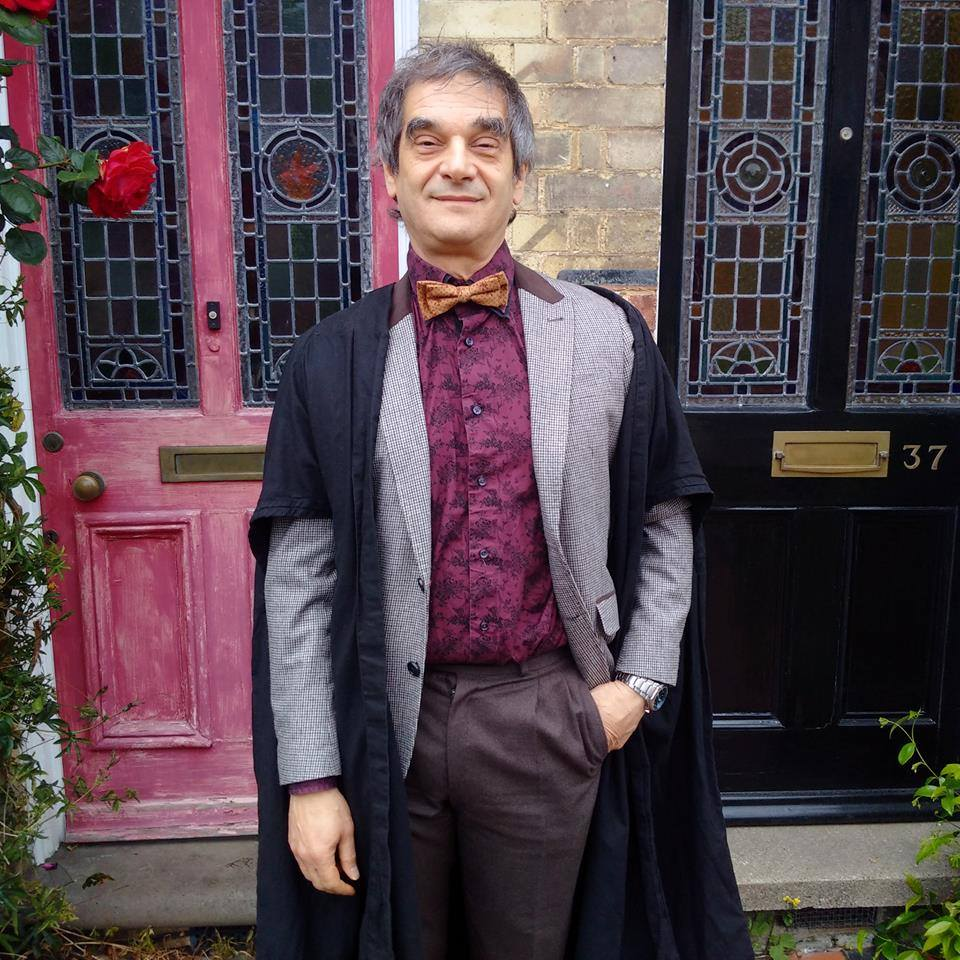
\includegraphics[scale=0.1]{larry.jpg}
\begin{itemize}
\item Lawrence Charles Paulson (Larry) is a professor at the University of Cambridge;\pause
\item His research is based around the interactive theorem prover Isabelle, which he introduced in 1986;\pause
\item He has worked on the verification of cryptographic protocols using inductive definitions;\pause
\item He has also formalized the constructible universe of Kurt Gödel;\pause

\end{itemize}
}

\frame{
\frametitle{Curiosities about Larry}
\begin{itemize}
\item He was one of the most cited researchers on a paper that demonstrated the existence of God by a machine on Gödel's world;\pause
\item He is a deep minded atheist;\pause
\item He has a page called: "Larry Paulson - Portrait of a God";\pause
\item http://www.geocities.ws/robrich18/Larry.html
\begin{center}

\includegraphics[scale=0.3]{LarryBond.jpg}
\end{center}
\end{itemize}
}

\frame{
\frametitle{Larry's Protocol Verification Time-line}
\begin{itemize}
\item Isabelle theorem prover;\pause
\begin{itemize}
\item General tool; \pause
\item Works with protocols since 1997;\pause
\end{itemize}
\item Many papers describing the Inductive Method he created;\pause
\item Many case studies, including:\pause
\begin{itemize}
\item Verification of SET protocol (6 papers)\pause
\item Kerberos (3 papers)\pause
\item TLS protocol\pause
\item Yahalom protocol, smart cards, etc\pause
\end{itemize}
\item Last work published in 2015: "Verifying multicast-based security protocols using the inductive method. Martina, J.E., Paulson, L.C."
\end{itemize}
}

\frame{
\frametitle{The Inductive Method}
\begin{itemize}
\item Starts with an informal protocol description;\pause
\item Out of that we extract:\pause
\begin{itemize}
\item An inductive abstract trace model;\pause
\item Correctness theorem about the traces;\pause
\end{itemize}
\item We then add the attacker inference rules;\pause
\item We state the goals ad theorems and lemmas;\pause
\item We prove the theorems inductively to demonstrate correctness.
\end{itemize}
}


\frame{
\frametitle{The Inductive Method Mechanics}
\begin{itemize}
\item Larry Paulson advocates a simple approach (called Inductive Method): \pause
\begin{itemize}
\item A protocol in a context describes a set of traces;\pause
\item These traces are defined inductively;\pause
\item A specification is again a property of traces;\pause
\item Checking requires proving that all the traces satisfy the property, by induction on the construction of the traces;\pause
\item Main point: these proofs are big, uninteresting, and better left to machines;\pause
\item Use a theorem prover (Isabelle)to write the proofs.
\end{itemize}
\end{itemize}
}

\frame{
\frametitle{Isabelle}
\begin{itemize}
\item Automated support for proof development, which supports:\pause
\begin{itemize}
\item Higher-order logic;\pause
\item Serves as a logical framework;\pause
\item Supports ZF set theory and HOL;\pause
\item Generic treatment of inference rules;\pause
\end{itemize}
\item Powerful simplifier, classical reasoner and connected tools;\pause
\item Strong support for inductive definitions.
\end{itemize}
}

\frame{
\frametitle{Inductive Method Support in Isabelle}
\begin{itemize}
\item There are several files to support security protocol verification in Isabelle:\pause
\begin{itemize}
\item \textit{Message.thy}, which specifies how the messages exchanged in security protocols are constructed, as well as the main operators we use within the method;\pause
\item \textit{Event.thy}, which inherits  from \textit{Message.thy} and accounts for the specification of the communication layer with the sending, receiving and noting events;\pause
\item \textit{Public.thy} which inherits from \textit{Event.thy}, which despite the narrowly chosen name, accounts for the specification of symmetric and asymmetric cryptographic primitives;\pause
\item We also have some other specialised theories for Smart-Cards, Threshold Cryptography and Multicast communication.
\end{itemize}
\end{itemize}
}

\frame{
\frametitle{Inductive Method Details - Agents}
\begin{mydef}{Agent datatype definition}\label{mydef:agent}
 \begin{isabelle}%
 \isacommand{datatype}\isamarkupfalse%
\isanewline
\ \ agent  {\isacharequal}\ Friend nat \isanewline
\ \ \ \ \ \ \ \ \ {\isacharbar} Server \isanewline
\ \ \ \ \ \ \ \ \ {\isacharbar} Spy
 \end{isabelle}%
\end{mydef}\pause
\begin{itemize}
\item First we have the definition of a friendly agent by the bijection explained above;\pause
\item The second category regards the trusted third party;\pause
\item Finally we have the attacker, which is categorised separately.
\end{itemize}
}

\frame{
\frametitle{Inductive Method Details - Cryptographic Keys}
\begin{mydef}{shrK function definition}\label{mydef:shrK}
 \begin{isabelle}%
 \isacommand{consts}\isamarkupfalse%
\isanewline
\ \ shrK    :: "agent => key"  \isanewline
\isacommand{specification} (shrK)\isamarkupfalse% 
\isanewline
\ \ inj\_shrK: "inj shrK"
 \end{isabelle}%
\end{mydef}\pause
\begin{itemize}
\item The specification of cryptographic keys in the Inductive Method starts with the introduction of a free type \textit{key} as a derivation of the type \textit{nat};\pause
\item A shared key is specified as an injective function taking an agent and returning a key.
\end{itemize}
}

\frame{
\frametitle{Inductive Method Details - Cryptographic Keys}
\begin{mydef}{invKey function definition}\label{mydef:invKey}
 \begin{isabelle}%
 \isacommand{consts}\isamarkupfalse%
\isanewline
\ \ invKey :: "key => key" \isanewline
\isacommand{specification} (invKey)\isamarkupfalse% 
\isanewline
\ \ invKey [simp]: "invKey (invKey K) = K"\isanewline
\ \ invKey\_symmetric: "all\_symmetric --> invKey = id"
 \end{isabelle}%
\end{mydef}\pause
\begin{itemize}
\item The function \textit{invKey}is a function from data type key to key specified by two rules:\pause
\begin{itemize}
\item The first rule is a simplification one that says that the double application of the function brings us back to the original value;\pause
\item The second rule establishes true if the function \textit{invKey} is equal to its identity.
\end{itemize} 
\end{itemize}
}

\frame{
\frametitle{Inductive Method Details - Cryptographic Keys}
\begin{mydef}{symKeys set definition}\label{mydef:symKeys}
 \begin{isabelle}%
 \isacommand{constdefs}\isamarkupfalse%
\isanewline
\ \  symKeys :: "key set"\isanewline
\ \  "symKeys == {K. invKey K = K}"
 \end{isabelle}%
\end{mydef}\pause
\begin{itemize}
\item The symmetric key set is defined as containing all keys where the inverse of the key by the application of the function \textit{invKey} is itself;\pause
\item  By stating \textit{K $\in$ symKeys $\wedge$ K $\notin$ range shrK} we can create a second class of symmetric keys that are not long-term so that it represents sessions keys in our protocols being verified.
\end{itemize}
}

\frame{
\frametitle{Inductive Method Details - Cryptographic Keys}
\begin{mydef}{Axiom for symmetric usage of shared keys}\label{mydef:axiomshrK}
 \begin{isabelle}%
 \isacommand{axioms}\isamarkupfalse%
\isanewline
\ \   sym\_shrK [iff]: "shrK X $\in$ symKeys"
 \end{isabelle}%
\end{mydef}\pause
\begin{itemize}
\item Establishs that our long-term keys are symmetric with an axiom.
\end{itemize}
}

\frame{
\frametitle{Inductive Method Details - Cryptographic Keys}
\begin{mydef}{publicKey definition}\label{mydef:publicKey}
 \begin{isabelle}%
 \isacommand{datatype}\isamarkupfalse
\isanewline
\ \ keymode = Signature | Encryption\isanewline
\isanewline
\isacommand{consts}\isamarkupfalse
\isanewline
\ \  publicKey :: "[keymode,agent] => key"\isanewline
\isanewline
 \isacommand{specification} (publicKey) \isamarkupfalse
 \isanewline
\ \  injective\_publicKey: \isanewline
 \ \ \ "publicKey b A = publicKey c A' ==> b=c \& A=A'"
 \end{isabelle}%
\end{mydef}\pause
}

\frame{
\frametitle{Inductive Method Details - Cryptographic Keys}
\begin{mydef}{privateKey  axiom definition}\label{mydef:privateKey}
 \begin{isabelle}%
 \isacommand{axioms}\isamarkupfalse
\isanewline
privateKey\_neq\_publicKey [iff]: \isanewline \ \ "privateKey b A $\neq$ publicKey c A'"
 \end{isabelle}%
\end{mydef}\pause
}

\frame{
\frametitle{Inductive Method Details - Cryptographic Keys}
\begin{mydef}{Public Key abbreviations }\label{mydef:keys}
 \begin{isabelle}%
 \isacommand{abbreviation}\isamarkupfalse
\isanewline
\ \ pubEK :: "agent => key" where \isanewline
\ \ "pubEK == publicKey Encryption" \isanewline
\ \  pubSK :: "agent => key" where \isanewline
\ \  "pubSK == publicKey Signature"\isanewline
\ \  privateKey :: "[keymode, agent] => key" where \isanewline
\ \  "privateKey b A == invKey (publicKey b A)"\isanewline
\ \  priEK :: "agent => key" where \isanewline
\ \  "priEK A == privateKey Encryption A"\isanewline
\ \  priSK :: "agent => key" where \isanewline
\ \  "priSK A == privateKey Signature A"\isanewline
 \end{isabelle}%
\end{mydef}
}

\frame{
\frametitle{Inductive Method Details  - Compromised Agents}
 \begin{mydef}{bad set definition }\label{mydef:bad}
 \begin{isabelle}%
 \isacommand{consts}\isamarkupfalse
\isanewline
\ \ bad    :: "agent set"	\isanewline
\isacommand{specification} (bad)\isamarkupfalse
\isanewline
\ \  Spy\_in\_bad     [iff]: "Spy $\in$ bad"\isanewline
\ \  Server\_not\_bad [iff]: "Server $\notin$ bad"
 \end{isabelle}%
\end{mydef}
}

\frame{
\frametitle{Inductive Method Details  - Messages}
 \begin{mydef}{msg datatype definition }\label{mydef:msg}
 \begin{isabelle}%
 \isacommand{datatype}
 \isamarkupfalse
\isanewline
\ \ msg = Agent  agent  \isanewline
\ \ \ \ \ \ \ \        | Number nat\isanewline
\ \ \ \ \ \ \ \        | Nonce  nat  \isanewline
\ \ \ \ \ \ \ \        | Key    key  \isanewline
\ \ \ \ \ \ \ \        | MPair  msg msg \isanewline
\ \ \ \ \ \ \ \        | Hash   msg \isanewline
\ \ \ \ \ \ \ \        | Crypt  key msg
 \end{isabelle}%
\end{mydef}
}

\frame{
\frametitle{Inductive Method Details  - Events}
\begin{mydef}{event datatype definition }\label{mydef:event}
 \begin{isabelle}%
 \isacommand{datatype}
 \isamarkupfalse
\isanewline
\ \ event = Says  agent agent msg  \isanewline
\ \ \ \ \ \ \ \        | Gets  agent       msg\isanewline
\ \ \ \ \ \ \ \        | Notes agent       msg  
 \end{isabelle}%
\end{mydef}
}

\frame{
\frametitle{Inductive Method Details  - Initial Knowledge}
\begin{mydef}{initState definition }\label{mydef:initState}
 \begin{isabelle}%
 \isacommand{consts}
 \isamarkupfalse
\isanewline
\ \ initState :: "agent => msg set"
\end{isabelle}%
\end{mydef}
}

\frame{
\frametitle{Inductive Method Details  - Initial Knowledge}
\begin{mydef}{Spy agent initial knowledge definition }\label{mydef:initSpy}
 \begin{isabelle}%
 \isacommand{primrec}
 \isamarkupfalse
\isanewline
\ \ initState\_Spy: \isanewline
\ \ \ \     "initState Spy        =    \isanewline
\ \ \ \         (Key ` invKey ` pubEK ` bad) $\cup$ \isanewline\ \ \ \ (Key ` invKey ` pubSK ` bad) $\cup$ \isanewline
\ \ \ \         (Key ` shrK ` bad) $\cup$ \isanewline
\ \ \ \         (Key ` range pubEK) $\cup$ (Key ` range pubSK)"
 \end{isabelle}%
\end{mydef}
}

\frame{
\frametitle{Inductive Method Details  - Knows}
\begin{mydef}{knows function definition }\label{mydef:knows_fun}
 \begin{isabelle}%
 \isacommand{consts}
 \isamarkupfalse
\isanewline
\ \ knows  :: "agent => event list => msg set"\isanewline
\isanewline
 \isacommand{primrec}
 \isamarkupfalse
\isanewline
\ \   knows\_Nil:   "knows A [] = initState A"\isanewline
\ \   knows\_Cons: \isanewline
\ \ \ \     "knows A (ev \# evs) = \isanewline
\ \ \ \        (if A = Spy then \isanewline
\ \ \ \ 	(case ev of \isanewline
\ \ \ \ \ \ 	   Says A' B X => insert X (knows Spy evs) \isanewline
\ \ \ \ \ \ 	 | Gets A' X => knows Spy evs \isanewline
\ \ \ \ \ \ 	 | Notes A' X  => \isanewline
\ \ \ \ \ \ \ \ 	     if A' $\in$ bad then insert X (knows Spy evs) \isanewline \ \ \ \ \ \ \ \ \ \ else knows Spy evs) 
 \end{isabelle}%
\end{mydef}
}

\frame{
\frametitle{Inductive Method Details  - Knows}
\begin{mydef}{knows function definition }\label{mydef:knows_fun}
 \begin{isabelle}%
 \isacommand{consts}
 \isamarkupfalse
\isanewline
\ \ \ \ 	else \isanewline
\ \ \ \ 	(case ev of \isanewline
\ \ \ \ \ \ 	   Says A' B X => \isanewline
\ \ \ \ \ \ \ \ 	     if A'=A then insert X (knows A evs) else knows A evs \isanewline
\ \ \ \ \ \ 	 | Gets A' X    => \isanewline
\ \ \ \ \ \ \ \ 	     if A'=A then insert X (knows A evs) else knows A evs \isanewline
\ \ \ \ \ \ 	 | Notes A' X    => \isanewline
\ \ \ \ \ \ \ \ 	     if A'=A then insert X (knows A evs) else knows A evs))"\isanewline
 \end{isabelle}%
\end{mydef}
}

\frame{
\frametitle{Inductive Method Details  - Operators}
\begin{mydef}{parts inductive set definition }\label{mydef:parts}
 \begin{isabelle}%
 \isacommand{inductive\_set}
 \isamarkupfalse
\isanewline
\ \ parts :: "msg set => msg set"\isanewline
\ \   for H :: "msg set"\isanewline
\ \   where \isanewline
\ \ \ \ \ \     Inj [intro]:               "X $\in$ H ==> X $\in$ parts H"\isanewline
\ \ \ \ \ \   | Fst:         "\{|X,Y|\}   $\in$ parts H ==> X $\in$ parts H"\isanewline
\ \ \ \ \ \   | Snd:         "\{|X,Y|\}   $\in$ parts H ==> Y $\in$ parts H"\isanewline
\ \ \ \ \ \   | Body:        "Crypt K X $\in$ parts H ==> X $\in$ parts H"
 \end{isabelle}%
\end{mydef}
}

\frame{
\frametitle{Inductive Method Details  - Operators}
\begin{mydef}{analz inductive set definition }\label{mydef:analz}
 \begin{isabelle}%
 \isacommand{inductive\_set}
 \isamarkupfalse
\isanewline
\ \ analz :: "msg set => msg set"\isanewline
\ \   for H :: "msg set"\isanewline
\ \   where \isanewline
\ \ \ \ \ \     Inj [intro,simp] :    "X $\in$ H ==> X $\in$ analz H"\isanewline
\ \ \ \ \ \   | Fst:     "\{|X,Y|\} $\in$ analz H ==> X $\in$ analz H"\isanewline
\ \ \ \ \ \   | Snd:     "\{|X,Y|\} $\in$ analz H ==> Y $\in$ analz H"\isanewline
\ \ \ \ \ \   | Decrypt [dest]: \isanewline
\ \ \ \ \ \ \ \ \             "[|Crypt K X $\in$ analz H; Key(invKey K): analz H|] ==>\isanewline\ \ \ \ \ \ \ \ X $\in$ analz H"\isanewline
 \end{isabelle}%
\end{mydef}
}

\frame{
\frametitle{Inductive Method Details  - Operators}
\begin{mydef}{synth inductive set definition }\label{mydef:synth}
 \begin{isabelle}%
 \isacommand{inductive\_set}
 \isamarkupfalse
\isanewline
\ \  synth :: "msg set => msg set"\isanewline
\ \   for H :: "msg set"\isanewline
\ \   where \isanewline
\ \ \ \ \ \     Inj    [intro]:   "X $\in$ H ==> X $\in$ synth H"\isanewline
\ \ \ \ \ \   | Agent  [intro]:   "Agent agt $\in$ synth H"\isanewline
\ \ \ \ \ \   | Number [intro]:   "Number n  $\in$ synth H"\isanewline
\ \ \ \ \ \   | Hash   [intro]:   "X $\in$ synth H ==> Hash X $\in$ synth H"\isanewline
\ \ \ \ \ \   | MPair  [intro]:   "[|X $\in$ synth H;  Y $\in$ synth H|] ==> \isanewline\ \ \ \ \ \ \ \ \{|X,Y|\} $\in$ synth H"\isanewline
\ \ \ \ \ \   | Crypt  [intro]:   "[|X $\in$ synth H;  Key(K) $\in$ H|] ==> \isanewline\ \ \ \ \ \ \ \ Crypt K X $\in$ synth H"
 \end{isabelle}%
\end{mydef}
}

\frame{
\frametitle{Inductive Method Details  - Operators}
\begin{mydef}{used function definition }\label{mydef:used}
 \begin{isabelle}%
 \isacommand{consts}
 \isamarkupfalse
\isanewline
\ \ used :: "event list => msg set"
\isanewline
 \isacommand{primrec}
 \isamarkupfalse
\isanewline
\ \   used\_Nil:   "used []         = (UN B. parts (initState B))"\isanewline
\ \   used\_Cons:  "used (ev \# evs) = \isanewline
\ \ \ \ 		     (case ev of \isanewline
\ \ \ \ \ \ 			Says A B X => parts \{X\} $\cup$ used evs \isanewline
\ \ \ \ \ \ 		      | Gets A X   => used evs \isanewline
\ \ \ \ \ \ 		      | Notes A X  => parts \{X\}  $\cup$ used evs)"\isanewline
 \end{isabelle}%
\end{mydef}
}

\frame{
\frametitle{Dummy Protocol}
\begin{figure}[htbp]
\begin{center}
\fbox{
\begin{tabular}{c c c c c c c }
1. & $A$ & $ \rightarrow$ & $B$ &:&  & $ \{|A, B, Na|\}_{K_{B}} $ \\
2. & $B$ & $\rightarrow$ & $A$ &:&  & $ \{| Na, Nb, K_{AB} |\}_{K_{A}} $ \\
3. & $A$ & $\rightarrow$ & $B$ &:&  & $ \{| Nb \}_{K_{AB}}$ \\
\end{tabular}
}
\caption{Example protocol}\label{fig:example_proto}
\end{center}
\end{figure}
}

\frame{
\frametitle{Dummy Protocol Specification}
\begin{mydef}{inductive definition of example protocol}\label{mydef:example_def}
 \begin{isabelle}%
 \isacommand{inductive\_set}
 \isamarkupfalse example :: "event list set"
 \isanewline
 where \isanewline
\ \ \ \ Nil:  "[] $\in$ example"\isanewline
 
\ \ \ \ |Fake:"[|evsf $\in$ example; X $\in$ synth(analz (knows Spy evsf))|]\isanewline
\ \ \ \ \          $ \Rightarrow$ Says Spy B X \# evsf $\in$ example"\isanewline
 
\ \ \ \ |EX1:  "[|evs1 $\in$ example;  Nonce NA $\notin$ used evs1|] \isanewline
\ \ \ \ \            $ \Rightarrow$Says A B (Crypt (pubK B)\{|Agent A, Agent B, Nonce NA|\}) \# \isanewline 
\ \ \ \ \             evs1  $\in$  example"\isanewline

 \end{isabelle}%
\end{mydef}
}

\frame{
\frametitle{Dummy Protocol Specification}
\begin{mydef}
 \begin{isabelle}%
\ \ \ \ |EX2:  "[|evs2 $\in$ example;  Nonce NB $\notin$ used evs2; \isanewline 
\ \ \ \ \ \ \ Key AB $\notin$ used evs1   \isanewline 
\ \ \ \ \ \ \ Says A' B (Crypt (pubK B)\{|Agent A, Agent B, Nonce NA|\}) \isanewline 
\ \ \ \ \ \ \  $\in$ set evs2|] \isanewline
\ \ \ \ \            $ \Rightarrow$Says B A (Crypt (pubK A) \{| Nonce NA, Nonce NB, Key AB|\}) \isanewline
\ \ \ \ \ \# evs2  $\in$  example"\isanewline
 
 \end{isabelle}%
\end{mydef}
}

\frame{
\frametitle{Dummy Protocol Specification}
\begin{mydef}
 \begin{isabelle}%

\ \ \ \ |EX3:  "[|evs3 $\in$ example; \isanewline
\ \ \ \ \ \ \ Says A B (Crypt (pubK B)\{|Agent A, Agent B, Nonce NA|\}) \isanewline 
\ \ \ \ \ \ \  $\in$ set evs3; \isanewline
\ \ \ \ \ \ \ Says B A (Crypt (pubK A) \{| Nonce NA, Nonce NB, Key AB|\}) \isanewline 
\ \ \ \ \ \ \  $\in$ set evs3 |] \isanewline
\ \ \ \ \            $ \Rightarrow$Says A B (Crypt (Key AB)\{| Nonce NB|\}) \# evs3  $\in$  example"\isanewline
 
 \end{isabelle}%
\end{mydef}
}


\frame{
\frametitle{Dummy Protocol Specification}
\begin{mydef}
 \begin{isabelle}%

\ \ \ \ |Oops: "[|evso $\in$ example; \isanewline 
\ \ \ \ \            Says B A (Crypt (pubK A) \{| Nonce NA, Nonce NB, Key AB|\}) \isanewline
\ \ \ \ \               $\in$ set evso|] \isanewline
\ \ \ \ \            $ \Rightarrow$ Notes Spy \{|Nonce NA, Nonce NB, Key AB|\}\# evso $\in$ example"
 
 \end{isabelle}%
\end{mydef}
}

\frame{
\frametitle{What to do next?}
\begin{itemize}
\item We describe the protocol goals as Theorems and Lemmas;\pause
\item We prove these inductively with the assistance of Isabelle;\pause
\item Proof tactics are known for most of the usual goals;\pause
\item The problem starts when you want to prove a new goal....
\end{itemize}
}

\frame{
\frametitle{Problems with the Inductive Method}
\begin{itemize}
\item Training someone to use it proficiently takes 2 years;\pause
\item Understanding Isabelle cryptic messages is painful\pause
\item The person carrying the verification need to be clever and seasoned with the tool, otherwise there will be pain;\pause
\item Too much freedom and power are sometimes difficult to use.
\end{itemize}
}

\frame{
	\frametitle{Discussion}
\begin{itemize}
\item What else can you foresee modelled using this strategy?\pause
\item Can this be extended?\pause
\item What this strategy can not do?
\end{itemize}
}

{
\usebackgroundtemplate{
\includegraphics[width=\paperwidth,
height=\paperheight]{../reusable_images/fundo_capa.png}}
\begin{frame}

{\LARGE Questions????}

\end{frame}
}

{
\usebackgroundtemplate{
\includegraphics[width=\paperwidth,
height=\paperheight]{../reusable_images/fundo_capa.png}}
\begin{frame}

\includegraphics[scale=0.8]{../reusable_images/cc_logo_arge.png}\hspace{0.5cm} 

\includegraphics[scale=0.95]{../reusable_images/by.png}

\vspace{1cm}
This work is licensed under the Creative Commons Attribution 4.0 International License. To view a copy of this license, visit http://creativecommons.org/licenses/by/4.0/.
\end{frame}
}

\end{document}